%-*- coding: utf-8 -*-
\documentclass[11pt,a4paper,french,twoside,openright]{article}
\usepackage[utf8]{inputenc}
\usepackage[T1]{fontenc}
\usepackage{graphicx}%pour insérer images et pdf entre autres
	\graphicspath{{images/}}%pour spécifier le chemin d'accès aux images
\usepackage[left=2.5cm,right=2.5cm,top=2.5cm,bottom=2.5cm]{geometry}%réglages des marges du document selon vos préférences ou celles de votre établissemant
\usepackage[Lenny]{fncychap}%pour de jolis titres de chapitres voir la doc pour d'autres styles.
\usepackage{babel}
\usepackage[babel=true]{csquotes} % csquotes va utiliser la langue définie dans babel

\usepackage{fancyhdr}%pour les entêtes et pieds de pages
	\setlength{\headheight}{14.2pt}% hauteur de l'entête
        \chead{\textbf{VITAMEAL}}
        \lhead{}
        \rhead{}
	\cfoot{Formation Ingénieur Informatique en alternance - Première année}
	\lfoot{\textbf{CNAM}}%
  	\rfoot{\textbf{\thepage/\pageref{LastPage}}}
 	\renewcommand{\headrulewidth}{0.4pt}%trait horizontal pour l'entête
  	\renewcommand{\footrulewidth}{0.4pt}%trait horizontal pour les pieds de pages

\usepackage[french]{nomencl}
\makenomenclature
\usepackage{hyperref}
\begin{document}
\pagestyle{fancy}

\begin{center}\bfseries\Huge
COMPTE RENDU DE RÉUNION
\end{center}

\textbf{Du      :} 03/03/2017 à 18h

\textbf{Objet   :} Avancement projet VITAMEAL

\textbf{Présents:} Nicolas SYMPHORIEN, Jean-Félix BENITEZ

\textbf{Absente :} Sonia OTHMANI

\textbf{Diffusion:} Nicolas SYMPHORIEN, Sonia OTHMANI, Jean-Félix BENITEZ

\hrulefill

\section{Méthode}
Après discussion, nous avons décidé d'adopter la méthode minimale pour sa simplicité de mise en oeuvre.
\begin{figure}[!ht]
\label{Mmin}
  \centering
      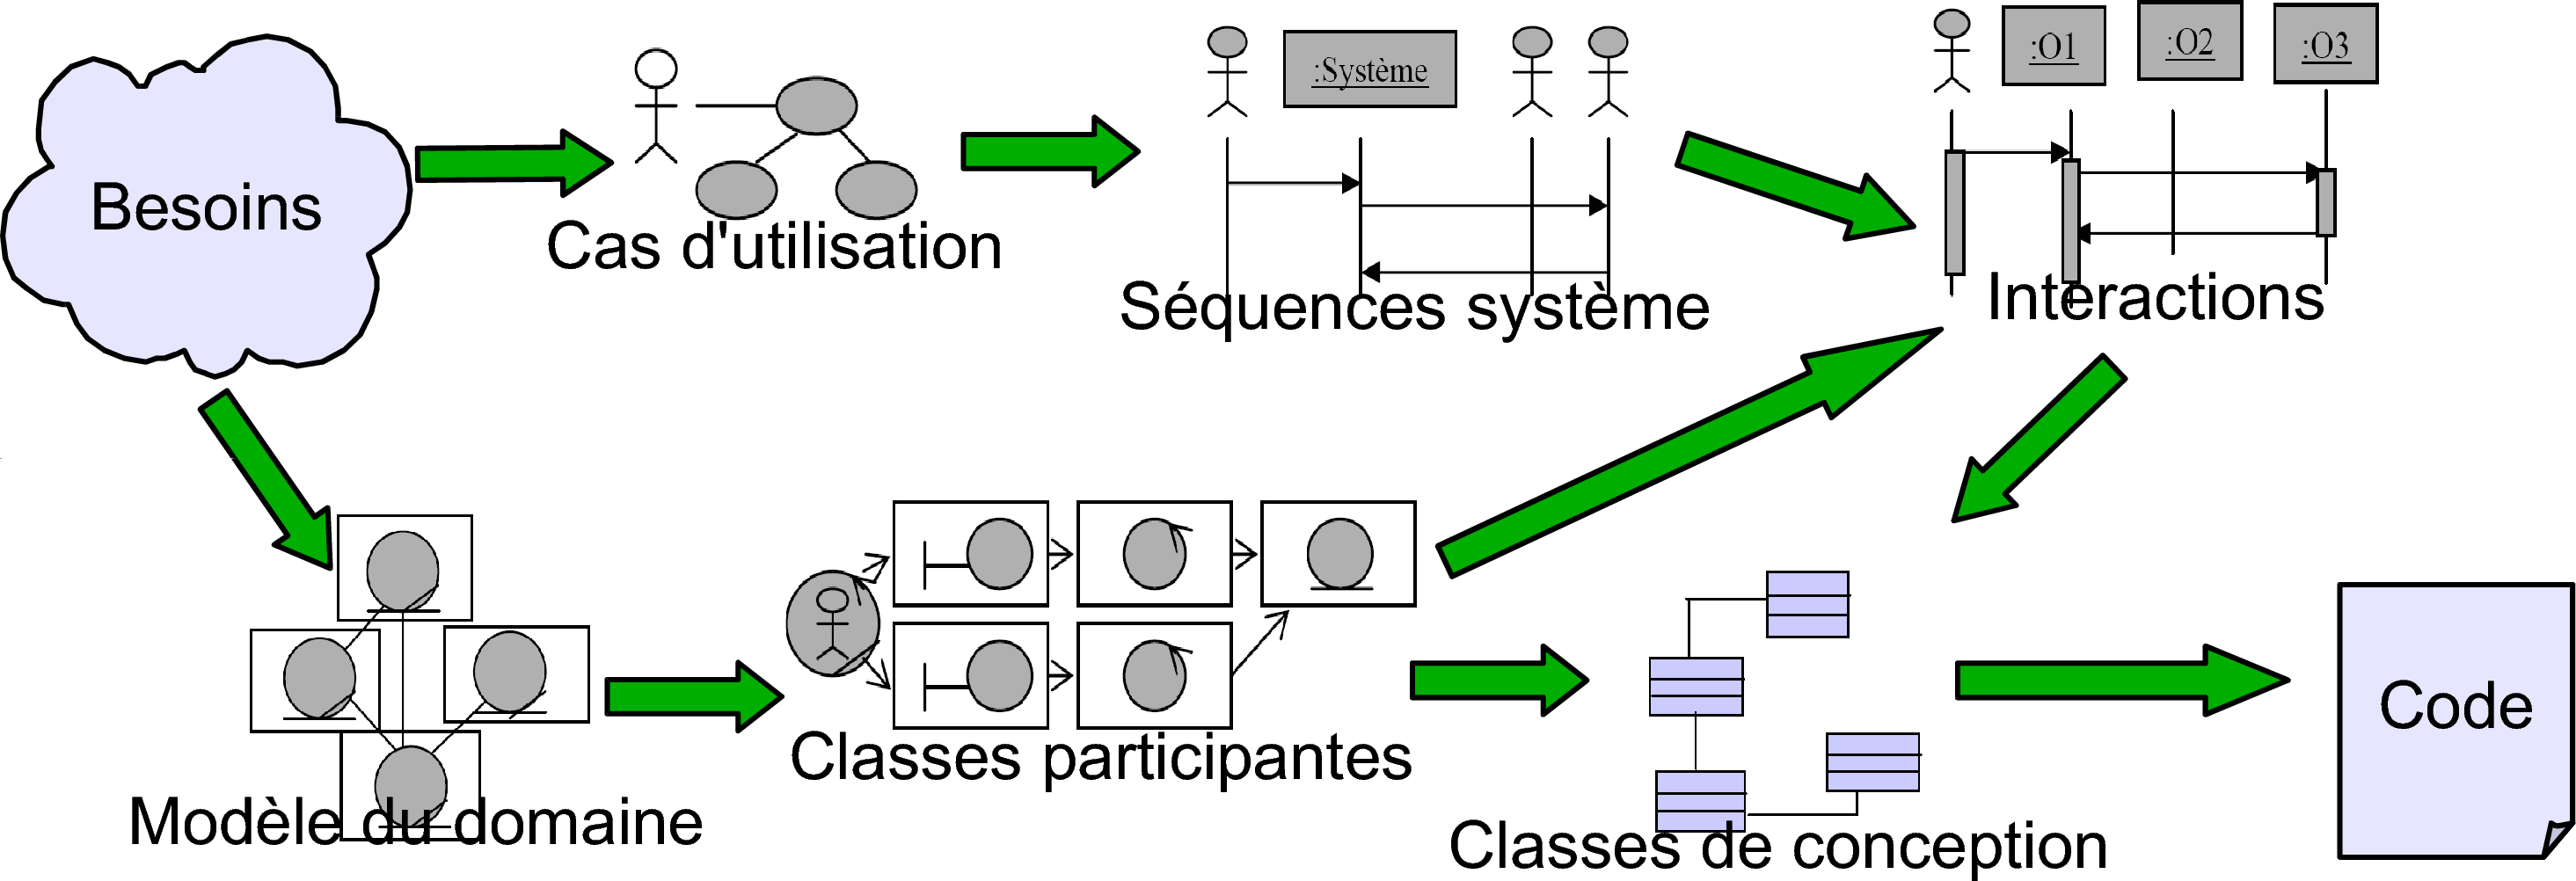
\includegraphics[width=0.5\textwidth]{MethodeMinimale}
\caption{Méthode minimale}
\end{figure}

\section{Planning}
Nous fixons la date de livraison à 2 semaines avant la présentation. La présentation du projet étant prévue pour le 14/09/2017; notre date de livraison est donc le 31/08/2017. Faute d'avoir suffisament d'expérience pour pourvoir évaluer de façon fiable la charge de travail que représente ce projet, nous allons nous baser sur le travail que nous pouvons alouer au quotidient à ce projet. Nous avons évalué notre capacité de travail à 1h par jours ouvré et 3h par jours de fin de semaine; ce qui fait un total de 11 heures chacun par semaine. Entre le 03 mars et le 31 août, il y a 25 semaines plus 4 jours; soit 279 heures chacuns.

Nous avons déduit de la figure~\ref{Mmin} , les cinq étapes de développement suivantes:
\begin{enumerate}
\item Cas d'utilisation et Modèle de domaine.
\item Séquences système et Classes participantes.
\item Diagramme d'intéractions.
\item Classes de conception.
\item Code.
\end{enumerate}
Pour évaluer la part de chaque étapes de développement, nous nous basons sur l'affirmation suivante \enquote{Aujourd'hui, un projet c'est 80\% de réflexion et 20\% de développement} (voir \url{http://www.logadap.fr/methodologie-creation-logiciel/}). Ainsi, le code va occuper 20\% de notre temps et les 4 étapes précédentes 80\%, soit 20\% par étapes.

C'est Jean-Félix qui prend en charge la définition du planning.

\section{Usine logicielle}
Nous avons d'ores et déjà adopté:
\begin{itemize}
\item \textbf{StarUML} pour la modélisation
\item \textbf{Eclipse} comme environnement de développement
\item \textbf{Git} comme gestionnaire de versions
\item \textbf{GitHub} comme dépôt de notre projet
\end{itemize}
C'est Nicolas qui prend en charge la définition de l'usine logicielle.

\section{Analyse des exigences}
Nous devons l'enrichir.

\section{Livraisons}
Nous avons convenus de livrer notre travails défini dans cette réunion le vendredi 10 mars.

\label{LastPage}
\end{document}
